%%
%% ****** ljmsamp.tex 13.06.2018 ******
%%
\documentclass[
11pt,%
tightenlines,%
twoside,%
onecolumn,%
nofloats,%
nobibnotes,%
nofootinbib,%
superscriptaddress,%
noshowpacs,%
centertags]%
{revtex4}
\usepackage{ljm}
\usepackage{listings}

\lstset{
language=C++,
basewidth=0.5em,
xleftmargin=45pt,
xrightmargin=45pt,
basicstyle=\small\ttfamily,
keywordstyle=\bfseries\underbar,
numbers=left,
numberstyle=\tiny,
stepnumber=1,
numbersep=10pt,
showspaces=false,
showstringspaces=false,
showtabs=false,
frame=trBL,
tabsize=2,
captionpos=t,
breaklines=true,
breakatwhitespace=false,
escapeinside={\%*}{*)}
}

\begin{document}

\titlerunning{Vectorization with AVX-512 instructions} % for running heads
\authorrunning{A.~A.~Rybakov and S.~S.~Shumilin} % for running heads
%\authorrunning{First-Author, Second-Author} % for running heads

\title{Vectorization of High-performance Scientific Calculations\\
Using AVX-512 Intruction Set}
% Splitting into lines is performed by the command \\
% The title is written in accordance with the rules of capitalization.

\author{\firstname{A.~A.}~\surname{Rybakov}}
\email[E-mail: ]{rybakov.aax@gmail.com}
\affiliation{Joint Supercomputer Center of the Russian Academy of Sciences - branch of Scientific Research Institute of System Analysis of the Russian Academy of Sciences, Leninsky prospect 32a, Moscow, 119334, Russia}

\author{\firstname{S.~S.}~\surname{Shumilin}}
\email[E-mail: ]{shumilin@jscc.ru}
\affiliation{Joint Supercomputer Center of the Russian Academy of Sciences - branch of Scientific Research Institute of System Analysis of the Russian Academy of Sciences, Leninsky prospect 32a, Moscow, 119334, Russia}
%\noaffiliation % If the author does not specify a place of work.

\firstcollaboration{(Submitted by G.~I.~Savin)} % Add if you know submitter.
%\lastcollaboration{ }

\received{June 13, 2018} % The date of receipt to the editor, i.e. December 06, 2017


\begin{abstract} % You shouldn't use formulas and citations in the abstract.
The article is devoted to the issues of vectorization of calculations for the processor Intel Xeon Phi Knights Landing (KNL). As objects for optimization, operations on low-dimensional matrices are considered. Such operations are common in the calculation codes from various fields of research, for example, when solving problems of gas dynamics. KNL are the newest processors in the Intel Xeon Phi line, they contain up to 72 cores and allow you to run applications using massive parallelism. They have a wide range of capabilities for efficiently performing supercomputer calculations, in particular, they support various memory modes and clustering modes. Often, the compiler does not cope with the task of creating highly efficient parallel vectorized code, which leads to performance losses. One of the reserves for improving code performance is the implementation of manual vectorization of the hottest code sections, which eventually results in the acceleration of the entire application. When using KNL processors, an important step to optimize the program is to enable special 512-bit vector instructions that can significantly speed up the executable code. Using 512-bit vector instructions allows you to process vectors containing 16 floating point elements. The presence of special combined FMA instructions allows combining the componentwise multiplication and addition of such vectors. To facilitate the process of manual vectorization of the program code, special intrinsiki functions are used, which are wrappers over the processor instructions. The use of vectorization of operations on matrices, performed using intrinsic functions, made it possible to reduce the execution time of these operations from 23% to 70% compared to the version built by the icc compiler and indicating the maximum level of optimization. The results obtained demonstrate additional reserves of application performance, which can be obtained using manual code optimization.
\end{abstract}

\subclass{68N19} % Enter 2010 Mathematics Subject Classification.

\keywords{Optimization, vectorization, AVX-512, predicated execution, intrinsics, application performance.} % Include keywords separeted by comma.

\maketitle

% Text of article starts here.

\section{Introduction}

Today, supercomputer technologies are increasingly used in various fields of science, industry and business. The use of simulation modeling using supercomputer calculations allows analyzing various situations and scenarios of interaction of objects of the surrounding world and obtaining results that are unavailable without the use of these tools. At the same time, the amount of data involved in supercomputer calculations is constantly increasing. The size of the calculated grids of hundreds of millions of cells is already common for launches on the supercomputers of the petaflops performance range [1, 2], and gradually there is a need to use grids containing billions of cells. Today, the most powerful supercomputer is the Chinese Sunway TaihuLight machine, which achieves a performance of 93 PFLOPS on the High Performance Linpack (HPL) benchmark [3]. In 2018, the emergence of several supercomputers with a performance in the range of 100-200 PFLOPS is expected, the most powerful of which will be IBM's Summit supercomputer, equipped with a Power9 processor and NVidia graphics processors with Volta architecture. According to some optimistic forecasts, the first exaflops supercomputer capable of performing $10^18$ floating point operations per second is possible by 2024 [4]. Along with increasing the computing power of supercomputers, questions arise about the effectiveness of their use. In particular, work is underway to improve the efficiency of data exchange systems between computing nodes [5, 6], to develop computational grid management technologies and to evenly distribute computations on a cluster [7, 8, 9], actively develop tools of programming languages ​​aimed at facilitating the creation of high-performance parallel code [10, 11].

The lowest-level direction of creating high-performance parallel executable code is vectorization of computations, which allows to directly use the hardware capabilities of calculators [12, 13]. In this paper, we consider the vectorization of small-size matrix operations for Intel Xeon Phi Knights Landing (KNL) processors. These operations are often found in computational problems and can take a significant part of the execution time of the calculation.

The Intel Xeon Phi x200 Knights Landing processor family is the second generation of the Intel Xeon Phi line and the first generation of solvers that act as a standalone processor (the first generation of the Knights Corner was a co-processor [14]). The first KNL processors were introduced in 2016. Each processor contains up to 36 active tiles, each of which consists of two cores and a L2 cache of 1 MB in size, which is common to the data of the two cores. Each core contains a VPU (Vector Processing Unit) that supports 512-bit vector instructions and a 64 KB L1 cache divided into equal by-size instruction cache and data cache of 32 KB each. Each core supports 4 threads, which gives a total of 288 logical processors per socket [15]. Although the frequency of each KNL core is lower than that of Intel Xeon server processors, such a number of execution threads and the presence of 512-bit vector instructions provide impressive peak performance in excess of 6 TFLOPS on single-precision operations.

The emergence of such a powerful hardware has opened up new possibilities for optimizing software used in supercomputer calculations. In [16], approaches were described that allowed using the vectorization for KNL to speed up the computational cores of the LAMMPS program code by up to 12 times compared to the non-vectorized version, which led to a general acceleration of solver runs by a factor of 2-3. One can note the successful application of vectorization to accelerate operations with sparse matrices of high dimensionality, which resulted in a fivefold acceleration on these operations [17]. Special features of KNL processors associated with the use of masked vector operations are used to vectorize cycles even with an unknown number of iterations and complex controls, as shown by the example of the vectorization of the Mandelbrot set construction code [18]. The work [19] describes the achievement of 6-fold acceleration achieved through the use of low-level optimization of computational codes for problems of nuclear physics. In [20], an example of the application of code vectorization is highlighted by removing the unlikely branch of execution from a hot inner loop.
However, despite the high potential of KNL, studies show that the acceleration achieved compared to launches on Intel Xeon processors of the Haswell and Broadwell generations rarely exceeds 1.5–2 times [21, 22]. This is partly due to the imbalance between peak bandwidth when working with memory and the intensity of arithmetic operations [23]. Active research is underway on the use of various memory modes and various clustering modes.

\section{Flat loops vectorization}

The simplest context for vectorization is a flat loop.
We will call a loop flat if it has the following properties.
First, it should not contain inter-iteration dependencies, that is, all loop iterations can be executed in parallel.
Secondly, within the iteration of the loop with number $i$ there can only be such memory access operations that read or write elements of arrays with indices $i$ (all references to memory can be reduced to the form $a[i]$).
A trivial example of a flat loop is the addition of two arrays.
In the most cases, flat loops containing only arithmetic operations are automatically compiled by the compiler and demonstrate multiple acceleration, since the AVX-512 instruction set contains vector analogues of all arithmetic operations.
The situation is more complicated with vectorization of flat loops containing specifities.
As examples of the flat loops specifities, conditional operators or control transfer commands can be given.
Such loops are also easily vectorized, but in practice the compiler often refuses to build a vector code due to a theoretical estimate of the possible acceleration.
The presence of a strongly branched control in a flat loop usually leads to the rejection of vectorization, in such cases the vector code must be built manually.
The more serious specifities that prevent the construction of an effective parallel code is the presence of nested loops or function calls in a flat loop.
In this case, the compiler is not able to perform vectorization, although using the intrinsic functions, optimization can also be performed in these cases.

Let us analyze in more detail the question of vectorization of flat loops.
Suppose that the vectorization uses vectors capable of containing $w$ primitive data elements, in this case we will call $w$ the vectorization width (AVX-512 vectors can contain 8 double elements or 16 float elements).
We will not consider a variant in which the loop body contains only arithmetic operations due to its triviality.
Let the considered flat loop contain $n$ iterations.
Then all iterations of this loop can be divided into $n / w$ groups by $w$ iterations, and each group can be considered separately (a residual group of iterations containing less than $w$ iterations is also possible; the presence of this group does not affect the optimization efficiency, it can be completed in the original form or vectorized using masks).
Thus, for simplicity, we can restrict ourselves to the consideration of flat cycles containing exactly $w$ iterations.

As a first example, we consider a flat loop whose body consists of a single linear section $block$, which is executed under the condition $cond_i$ with probability $p$ and has a length $t$ (Fig.~\ref{fig:flat_loop_1}, a).
In this case, the length of a linear section is understood to be a characteristic proportional to the execution time of a given linear section (the number of operators or machine instructions).
The total number of operations contained in the loop is $ptw$ (in this case, we assume that the auxiliary instructions related to the calculation of the condition and the provision of control can be neglected).
If the probability that the condition $cond_i$ is satisfied is low enough, then we can only stop at the vectorization of this condition and perform the whole loop under vectorized condition $vcond$.
This transformation will be called the vectorization of the condition (Fig.~\ref{fig:flat_loop_1}, b).
Moreover, the probability that the condition $vcond$ turns out to be instinctive is $1 - (1 - p) ^ w$ (corresponds to the fact that at least one of the $w$ elementary conditions is true).
The total number of operations in the loop from this conversion will not change (the $cond_i$ and $vcond$ conditions are not independent) and will remain equal to $ptw$, but the number of auxiliary operations and control operations will be reduced.
To vectorize the entire loop, it is necessary to convert the program code into a predicate code, in which each instruction of the linear section $block$ is executed under the predicate $cond_i$, then all the instructions of the linear section can be replaced by vector analogs executed under the vector predicate $vcond$ (Fig.~\ref{fig:flat_loop_1}, c).
The number of operations of a fully vectorized loop is simply $t$.
At the same time, it is also not forbidden to use $vcond$ checking for voidness before executing vectorized code in order to avoid executing code blocks with empty masks (Fig.~\ref{fig:flat_loop_1}, d).
In this case, the number of loop operations will be reduced by $1 - (1 - p) ^ w$ times, since the addition of a condition will cut off the execution of vector operations with an empty mask.

\begin{figure}[h]
\setcaptionmargin{5mm}
\onelinecaptionstrue
\includegraphics[width=0.62\textwidth]{pics/if_vectorization.pdf}
\captionstyle{normal}\caption{Example of flat loop with single linear section $block$ under condition $cond_i$.}
\label{fig:flat_loop_1}
\end{figure}

As another example, consider a flat loop whose body is an if-else statement.
Without loss of generality, we assume that the branch executed by the if-condition ($block_1$) is more likely than its alternative ($block_2$), that is $p \ge 1 - p$, or $p \ge \frac{1}{2}$.
The lengths of the linear sections in this example are $t_1$ and $t_2$, respectively (Fig.~\ref{fig:flat_loop_2}, a).
In addition, we will assume that the $block_1$ linear section is suitable for vectorization in any case, and a vector code is constructed for it (otherwise, the optimization of this code loses its meaning).
The total number of operations performed during the loop operation is calculated as the mathematical expectation of the number of operations per iteration multiplied by the number of iterations of the loop, that is $(pt_1 + (1 - p) t_2) w$.
In real computational problems, it often happens that an unlikely branch in such cycles does not lend itself to vectorization or this requires considerable effort.
Such unlikely branches contain processing of extremely rare exceptions or unexpected situations.
In such cases, it is natural to vectorize only the probable branch, and leave the alternative under the vectorized condition (Fig.~\ref{fig:flat_loop_2}, b).
Such a half vectorized loop will contain $t_1 + (1 - p) t_2w$ operations.
In the case of a complete vectorization of the loop body, both linear sections fall under opposite predicates ($vcond$, ${\sim}vcond$) and the loop body is completely freed from the control transfer commands (Fig.~\ref{fig:flat_loop_2}, c).
The number of executed instructions in a loop for a fully vectorized code is $t_1 + t_2$.
As a last action, we apply the addition of checking the condition $~vcond$ for an unlikely branch to exclude the execution of operations with empty masks (Fig.~\ref{fig:flat_loop_2}, d).
Since the probability of executing an alternative is $1 - p ^ w$, the final number of operations performed for a fully vectorized cycle with checking the vectorized condition for an alternative is $t_1 + (1 - p ^ w) t_2$.

\begin{figure}[h]
\setcaptionmargin{5mm}
\onelinecaptionstrue
\includegraphics[width=0.65\textwidth]{pics/if_else_vectorization.pdf}
\captionstyle{normal}\caption{Example of flat loop with if-else statement.}
\label{fig:flat_loop_2}
\end{figure}

The Table~\ref{tab:flat} contains data on the number of operations performed for the two considered examples of flat loops, in which the loop body consists of one if-condition and one if-else-construction.

\begin{table}[!h]
\setcaptionmargin{0mm}
\onelinecaptionsfalse
\captionstyle{flushleft}
\caption{Operations count for if and if-else statements vectorization in flat loops.}
\bigskip
\begin{tabular}{|c|c|c|c|}
\hline
if statement & operations count & if-else statement & operations count \\
\hline
a) & $ptw$ & a) & $\left( pt_1 + (1 - p)t_2 \right)w$ \\
b) & $ptw$ & b) & $t_1 + (1 - p)t_2w$ \\
c) & $t$ & c) & $t_1 + t_2$ \\
d) & $\left( 1 - (1 - p)^w \right)t$ & d) & $t_1 + (1 - p^w)t_2$ \\
\hline
\end{tabular}
\label{tab:flat}
\end{table}

We will analyze only the second example with the if-else statement (the first example is treated similarly).
A fully vectorized loop is more profitable than a loop with a vectorized condition, if it contains fewer operations, that is, if the condition $t_1 + t_2 \le t_1 + (1 - p) t_2w$, or $(1 - p) w \ge 1$ is satisfied.
Thus, for the benefit of vectorization, either a high vectorization width, or a high probability of an alternative.
If we consider the application of checking vectorized conditions for a fully vectorized loop body, then we obtain the condition $t_1 + (1 - p ^ w) t_2 \le t_1 + (1 - p) t_2w$, which translates into $1 - p ^ w \le (1 - p) w$.
This condition is equivalent to the following:

\begin{equation}
\sum_{i = 0}^{w - 1}{p^i} \le w
\end{equation}

This condition is obviously satisfied, since $p <= 1$, and the total terms count is exactly $w$.
Thus, we have obtained that using a fully vectorized loop body with a preliminary check of a vectorized condition for an unlikely branch is always more beneficial than using the original version of the code or condition vectoring.
Note that this conclusion is true only under the assumption that the $block_1$ linear segment is probable, and a vector code is always built for it.

We can consider the general case of vectorization of a flat loop containing an arbitrary number of alternatives.
Let the loop body contain $n$ alternatives (with numbers from 0 to $n - 1$), each of which is executed with probability $p_i$.
In this case, we can neglect the operations of calculating conditions.
It is also known that each alternative has a length $t_i$.
It is required to understand the conditions under which the use of vectorization is beneficial, as well as the application of checking vectorized conditions for a vector code.
As in the previous examples, you can calculate the total number of running operations for a non-vectorized code; it is equal to the mathematical expectation of the number of operations per iteration of the loop multiplied by the number of iterations.

\begin{equation}
T = \left( \sum_{i = 0}^{n - 1}{p_it_i} \right) w
\end{equation}

With a complete loop vectorization, the number of vector operations is of course equal to the sum of the lengths of all linear sections $t_i$.
Thus, the condition of the advantage of vectorization is the following equation:

\begin{equation}
\sum_{i = 0}^{n - 1}{t_i(p_iw - 1)} \ge 0
\end{equation}

In particular, it follows from this equation that if the loop body contains a large number of alternative execution branches with probabilities less than $1 / w$, then vectoring of this loop cannot be beneficial.
When adding checks of vectorized conditions for each of the cycle alternatives, we obtain the following equation for the advantage of vectorization.

\begin{equation}
\sum_{i = 0}^{n - 1}{t_i \left( p_iw - 1 + (1 - p_i) ^w \right) } \ge 0
\end{equation}

Consider this formula more closely.
With a large number of alternatives, their probabilities are close to zero, so the term $(1 - p_i) ^ w$ is a positive value not much less than one.
From this we can conclude that the use of vectorized checks before performing vector versions of alternatives in the body of a flat loop significantly increase the effect of vectorization.
At least the theoretical estimates made in our assumptions indicate the benefits of applying such transformations.
However, one should not forget that vector commands generally execute more slowly than their scalar counterparts.
Moreover, the derivation of theoretical estimates did not take into account the influence of management operations and preparation of conditions, did not take into account the fact of the presence of possible dependencies between the calculation of conditions for various alternatives.

\section{Matrix operations vectorization}

In modern numerical methods used in high-performance computing, a special place is occupied by operations with vectors and matrices.
Such operations include calculating the scalar product of two vectors, multiplying the matrix by the vector, finding the inverse matrix, decomposing the matrix, and other operations.
In particular, the most frequently used operation is the multiplication of two matrices.
Obtaining the product of two matrices, in which the scalar product of each row of the first matrix and each column of the second matrix is calculated, is a rather difficult operation that can take up a significant part of the total program execution time.
The presence of effective approaches to the implementation of this operation is necessary to ensure the effective operation of program codes using matrix calculations.
The capabilities of the AVX-512 instruction set allow to create efficient code for implementations of matrix operations, which provides significant acceleration of applications, which use them.
In this section, we will consider the operations of multiplying small-size matrices (having sizes $8 \times 8$, $7 \times 7$, $6 \times 6$ and $5 \times 5$ elements).
Operations with such matrices take, for example, up to 40\% of the total operating time of the indigenous Russian RANS/ILES calculation codes used in the modeling of unsteady turbulent flows \cite{Lyub_RANS_ILES, Ben_Lyub_Chest_RANS_ILES}.
For reasons of alignment in memory, these matrices are considered as submatrices of a matrix of size $8 \times 8$ elements, as shown in Fig.~\ref{fig:matrices_8x8_7x7_6x6_5x5}.

\begin{figure}[h]
\setcaptionmargin{5mm}
\onelinecaptionsfalse % if the caption is multiline
\includegraphics[width=0.95\textwidth]{pics/matrices_8x8_7x7_6x6_5x5.pdf}
\captionstyle{normal}\caption{Matrices of size $8 \times 8$, $7 \times 7$, $6 \times 6$, $5 \times 5$ located inside the matrix of size $8 \times 8$. \\ The number of elements, and the number of addition and multiplication operations \\ required to perform the multiplication of two matrices of a given size.}\label{fig:matrices_8x8_7x7_6x6_5x5}
\end{figure}

We will compare the two approaches to implementing the multiplication of matrices of size $8 \times 8$, extend these approaches to smaller matrices and obtain the results of the comparison of the performance of the considered approaches.
The multiplication logic of two matrices is that the results of the pairwise scalar product of all rows of the first matrix and all columns of the second matrix form the elements of the resulting matrix.

First, we consider a direct approach to matrix multiplication, in which we will directly operate with the rows of the first matrix and the columns of the second matrix.
The matrices in programming language C, represented as multidimentional arrays, are located in memory row by row, so for reading matrix row it is neeeded to use the operation of consequental loading from memory (\texttt{load}), and for reading matrix column it is needed to use operation of loading data elements with arbitrary offsets from base address (\texttt{gather}).
We consider matrices whose elements are real single-precision values, therefore one \texttt{zmm} register with which commands from the instruction set AVX-512 operate, contains 16 elements of such matrix.
Thus, the AVX-512 allows to load two rows or two columns of a matrix using one command.

Fig.~\ref{fig:mmult_1} illustrates the implementation of this approach.
First of all, we note that the left matrix (matrix $A$) is completely loaded into 4 vectors $A_1$, $A_2$, $A_3$, $A_4$ (each vector contains two adjacent rows of the matrix).
This can be done using the usual instructions for reading sequentially located data from the memory (\texttt{load}).
Next, we present a scheme for calculating two adjacent columns of the resulting matrix (columns numbered $j$ and $h = j + 1$).
Two adjacent columns of the right matrix (matrix $B$) are loaded in the forward and reverse order into the vectors $B_j$ and $B_h$ (using the instructions \texttt{gather} for reading data from the memory and \texttt{permute} for placing \texttt{zmm} vector halves in reverse order, Fig.~\ref{fig:mmult_1}, 1).
Next, the operations of the elementwise multiplication of the vectors $B_j$ and $B_h$ by all the vectors, in which the matrix $A$ is loaded, are performed.
The results of these multiplications are 8 vectors $M_0$ - $M_7$ (Fig.~\ref{fig:mmult_1}, 2).
Each half of the $M_i, i \in [0, 7]$ vector (lower or high) contains elements, the sum of which forms one of the elements of the resulting matrix.
The calculation of the sum of the halves of all 8 vectors can be performed in parallel, with the result that all 16 required resulting values will be located in one vector (Fig.~\ref{fig:mmult_1}, 3).
Finally, the resulting 16 values are written into the columns with the $j$ and $h$ numbers of the resulting matrix, using command \texttt{scatter} (Fig.~\ref{fig:mmult_1}, 4).


\begin{figure}[h]
\setcaptionmargin{5mm}
\onelinecaptionsfalse % if the caption is multiline
\includegraphics[width=0.95\textwidth]{pics/mmult_1.pdf}
\captionstyle{normal}\caption{Scheme of two matrices multiplication with direct reading of rows and columns \\ of matrices and parallel computation of their pairwise scalar products.}\label{fig:mmult_1}
\end{figure}

Let us pay special attention to the parallel calculation of the sums of the \texttt{zmm} vectors halves.
AVX-512 instruction set does not contain horizontal operations of vectors elements addition, therefore, these operations have to be emulated by adding a vector with its copy, in which the elements are rearranged as needed.
For these purposes, we will use specially implemented macros consisting of \texttt{swizzle}, \texttt{permute}, \texttt{blend} and \texttt{add} instructions and allowing to add adjacent vector elements, pairs of adjacent vector elements and fours of adjacent vector elements, depending on the masks submitted.
Below is a listing of the implementation of these macros.

\begin{lstlisting}
#define SWIZ_2_ADD_2_BLEND_1(X, Y, SWIZ_TYPE, BLEND_MASK)         \
    _mm512_mask_blend_ps(BLEND_MASK,                              \
                         ADD(X, _mm512_swizzle_ps(X, SWIZ_TYPE)), \
                         ADD(Y, _mm512_swizzle_ps(Y, SWIZ_TYPE)))
#define PERM_2_ADD_2_BLEND_1(X, Y, PERM_TYPE, BLEND_MASK)              \
    _mm512_mask_blend_ps(BLEND_MASK,                                   \
                         ADD(X, _mm512_permute4f128_ps(X, PERM_TYPE)), \
                         ADD(Y, _mm512_permute4f128_ps(Y, PERM_TYPE)))
\end{lstlisting}

The \texttt{\_mm512\_swizzle\_ps} intrinsic is designed to rearrange the vector elements inside 128-bit quarters (composed of 4 single-precision floating-point elements), the \texttt{\_mm512\_permute4f128\_ps} command shuffles the 128-bit quarters themselves, and the \texttt{\_mm512\_mask\_blend\_ps} intrinsic performs the merging of two vectors using a mask.
To calculate the elements sums for 16 halves of 8 registers \texttt{zmm}, the use of 7 such macros is required (4 operations for the first level of merging, 2 operations for the second level of merging and the last operation for obtaining the resulting vector $M_2$, as shown on the Fig.~\ref{fig:mmult_1}, 3).
Since the scheme shown in Fig.~\ref{fig:mmult_1} provides the calculation of two adjacent columns of the resulting matrix, four such iterations are required to obtain the entire matrix.
Below is a complete source code listing of the function \texttt{mul\_8x8}, implementating matrices multiplication in accordance with the described approach.

\begin{lstlisting}
void mul_8x8(float * __restrict a, float * __restrict b,
             float * __restrict r)
{
    ........................................
    __m512 bj, bj2,
           m0, m1, m2, m3, m4, m5, m6, m7;

    // Indices for matrix columns.
    __m512i ind_cc = _mm512_set_epi32(7*V8+1, 6*V8+1, 5*V8+1, 4*V8+1,
                                      3*V8+1, 2*V8+1,   V8+1,      1,
                                      7*V8  , 6*V8  , 5*V8  , 4*V8  ,
                                      3*V8  , 2*V8  ,   V8  ,      0);
    __m512i ind_st = _mm512_set_epi32(7*V8  , 7*V8+1, 5*V8  , 5*V8+1,
                                      3*V8  , 3*V8+1,   V8  ,   V8+1,
                                      6*V8+1, 6*V8  , 4*V8+1, 4*V8  ,
                                      2*V8+1, 2*V8  ,      1,      0);

    // Load the rows of matrix "a".
    __m512 a0 = LD(&a[0]);
    ........................................
    __m512 a3 = LD(&a[6 * V8]);

    // Matrix "b" columns loop.
    for (int j = 0; j < V8; j += 2)
    {
        bj = _mm512_i32gather_ps(ind_cc, &b[j], _MM_SCALE_4);
        bj2 = _mm512_permute4f128_ps(bj, _MM_PERM_BADC);

        // Matrix "a" rows on matrix "b" columns multiplication.
        m0 = MUL(a0, bj);
        m1 = MUL(a0, bj2);
        ........................................
        m6 = MUL(a3, bj);
        m7 = MUL(a3, bj2);

        // Parallel calculation of vectors sums of elements.
        m0 = SWIZ_2_ADD_2_BLEND_1(m0, m1, _MM_SWIZ_REG_CDAB, 0xAAAA);
        m1 = SWIZ_2_ADD_2_BLEND_1(m2, m3, _MM_SWIZ_REG_CDAB, 0xAAAA);
        m2 = SWIZ_2_ADD_2_BLEND_1(m4, m5, _MM_SWIZ_REG_CDAB, 0xAAAA);
        m3 = SWIZ_2_ADD_2_BLEND_1(m6, m7, _MM_SWIZ_REG_CDAB, 0xAAAA);
        m0 = SWIZ_2_ADD_2_BLEND_1(m0, m1, _MM_SWIZ_REG_BADC, 0xCCCC);
        m1 = SWIZ_2_ADD_2_BLEND_1(m2, m3, _MM_SWIZ_REG_BADC, 0xCCCC);
        m2 = PERM_2_ADD_2_BLEND_1(m0, m1, _MM_PERM_CDAB, 0xF0F0);

        // Store the result.
        _mm512_i32scatter_ps(&r[j], ind_st, m2, _MM_SCALE_4);
    }
\end{lstlisting}

The experiments carried out demonstrated the effectiveness of this approach in relation to matrices of size $16 \times 16$.
However, using smaller matrices, a decrease in performance was observed.
The main reason for this is the use of slow multiple memory access operations with arbitrary offsets.
To eliminate this drawback, we consider another approach, in which calls to memory are performed only by sequential addresses.
At the same time, we note that this approach is applicable only for matrices of size no more than $8 \times 8$, since it requires a large number of \texttt{zmm} registers.
In the event of a shortage of \texttt{zmm} registers, these registers are immediately dumped into memory, which causes extra store and load commands (so-called spill/fill operations appear) and leads to a catastrophic performance decrease.

So, when forming another approach to the multiplication of small-format matrices, we will consider the removal of multiple memory access operations as well as the use of special combined operations, which allow the expression $\pm a \cdot b \pm c$ to be calculated in one operation, as the main goals.
We write the formulas for the $i$-th column of the resulting matrix:

\begin{equation}
\begin{cases}
r_{i0} = a_{i0}b_{00} + a_{i1}b_{10} + \ldots + a_{i7}b_{70} \\
\ldots \\
r_{i7} = a_{i0}b_{07} + a_{i1}b_{17} + \ldots + a_{i7}b_{77} \\
\end{cases}
\end{equation}

or in vector form

\begin{equation}
\overline{r_i} = a_{i0}\overline{b_0} + a_{i1}\overline{b_1} + \ldots + a_{i7}\overline{b_7} \\
\end{equation}

Similar expressions can be written for the row with the number $i + 1$:

\begin{equation}
\begin{cases}
r_{i+1,0} = a_{i+1,0}b_{00} + a_{i+1,1}b_{10} + \ldots + a_{i+1,7}b_{70} \\
\ldots \\
r_{i+1,7} = a_{i+1,0}b_{07} + a_{i+1,1}b_{17} + \ldots + a_{i+1,7}b_{77} \\
\end{cases}
\end{equation}

or in vector form

\begin{equation}
\overline{r_{i+1}} = a_{i+1,0}\overline{b_0} + a_{i+1,1}\overline{b_1} + \ldots + a_{i+1,7}\overline{b_7} \\
\end{equation}

Considering that the \texttt{zmm} registers contain 16 float elements, it is advisable to combine the above formulas into one, written in vector form as follows:

\begin{equation}
\begin{pmatrix} \overline{r_i} \\ \overline{r_{i+1}} \end{pmatrix}
=
\left(
\begin{pmatrix} \overline{a_{i0}} \\ \overline{a_{i+1,0}} \end{pmatrix}
\circ
\begin{pmatrix} \overline{b_0} \\ \overline{b_0} \end{pmatrix}
\right)
+
\left(
\begin{pmatrix} \overline{a_{i1}} \\ \overline{a_{i+1,1}} \end{pmatrix}
\circ
\begin{pmatrix} \overline{b_1} \\ \overline{b_1} \end{pmatrix}
\right)
+
\ldots
+
\left(
\begin{pmatrix} \overline{a_{i7}} \\ \overline{a_{i+1,7}} \end{pmatrix}
\circ
\begin{pmatrix} \overline{b_7} \\ \overline{b_7} \end{pmatrix}
\right)
\end{equation}

where $\begin{pmatrix} \overline{r_i} \\ \overline{r_{i+1}} \end{pmatrix}$ denotes the combined vector consisting of the vectors $\overline{r_i}$ and $\overline{r_{i+1}}$, $\begin{pmatrix} \overline{b_j} \\ \overline{b_j} \end{pmatrix}$ denotes the combined vector consisting of two copies of the vector $\overline{b_j}$, and the expression $\begin{pmatrix} \overline{a_{ij}} \\ \overline{a_{i+1,j}} \end{pmatrix}$ denotes a vector, the first 8 elements of which are equal to $a_{ij}$, and the remaining 8 elements are equal to $a_{i+1,j}$ (``$\circ$'' is Hadamard product, or elementwise product of vectors).
Note that the combined vector obtained according to this formula $\begin{pmatrix} \overline{r_i} \\ \overline{r_{i+1}} \end{pmatrix}$ is located in the memory sequentially, and it can be recorded into memory using the \texttt{store} instruction.
In this case, we assume that the value of $i$ is even, that is, the vector $\begin{pmatrix} \overline{r_i} \\ \overline{r_{i+1}} \end{pmatrix}$ is properly aligned in the memory.
Other combined vectors in this expression are obtained using the \texttt{permute} instruction (intrinsic function \texttt{\_mm512\_permutexvar\_ps}) applied to the corresponding loaded adjacent rows of the $A$ and $B$ matrices.
Thus, the implementation of the above formula does not require the use of slow \texttt{gather}/\texttt{scatter} instructions, since we don't read or write the columns of the matrices (calculations are performes only with rows).
After the required vectors are formed, we need to perform their pairwise elementwise multiplication, and then add them into one vector (8 operations of elementwise multiplication, 7 addition operations).
These actions can be performed using combined operations \texttt{fmadd}.
To calculate the value $\begin{pmatrix} \overline{r_i} \\ \overline{r_{i+1}} \end{pmatrix}$, we need 8 vector operations (1 operation \texttt{mul} and 7 operations \texttt{fmadd}).

Below is a complete source code listing of the function \texttt{mul\_8x8}, implementating matrices multiplication in accordance with the described approach.

\begin{lstlisting}
void mul_8x8(float * __restrict a, float * __restrict b,
             float * __restrict r)
{
    ........................................
    // Vector duplication indices.
    __m512i ind_df = _mm512_set_epi32( 7,  6,  5,  4,  3,  2, 1, 0,
                                       7,  6,  5,  4,  3,  2, 1, 0);
    __m512i ind_ds = _mm512_set_epi32(15, 14, 13, 12, 11, 10, 9, 8,
                                      15, 14, 13, 12, 11, 10, 9, 8);

    // Load and duplicate all rows of the matrix "b".
    __m512 b0 = LD(&b[0]);
    __m512 b1 = _mm512_permutexvar_ps(ind_ds, b0);
    b0 = _mm512_permutexvar_ps(ind_df, b0);
    ........................................
    __m512 b6 = LD(&b[6 * V8]);
    __m512 b7 = _mm512_permutexvar_ps(ind_ds, b6);
    b6 = _mm512_permutexvar_ps(ind_df, b6);

    // Load all rows of the matrix "a".
    __m512 a0 = LD(&a[0]);
    ........................................
    __m512 a6 = LD(&a[6 * V8]);

    // 8 indices for select elements from matrix "a".
    __m512i ind_0 = _mm512_set_epi32( 8,  8,  8,  8,  8,  8,  8,  8,
                                      0,  0,  0,  0,  0,  0,  0,  0);
    ........................................
    __m512i ind_7 = _mm512_set_epi32(15, 15, 15, 15, 15, 15, 15, 15,
                                      7,  7,  7,  7,  7,  7,  7,  7);

// Main block of operations.
#define BLOCK(N, A)                           \
    ST(&r[N * V8],                            \
      FMADD(PERMXV(ind_0, A), b0,             \
        FMADD(PERMXV(ind_1, A), b1,           \
          FMADD(PERMXV(ind_2, A), b2,         \
            FMADD(PERMXV(ind_3, A), b3,       \
              FMADD(PERMXV(ind_4, A), b4,     \
                FMADD(PERMXV(ind_5, A), b5,   \
                  FMADD(PERMXV(ind_6, A), b6, \
                    MUL(PERMXV(ind_7, A), b7)))))))));

    // Calculate and store the result.
    BLOCK(0, a0);
    BLOCK(2, a2);
    BLOCK(4, a4);
    BLOCK(6, a6);

#undef BLOCK

}
\end{lstlisting}

To implement the matrices multiplication in this function first we perform a full load of both matrices $A$ and $B$.
This requires 8 \texttt{load} operations, since two adjacent rows of the matrix are loaded in one operation.
Next, we need to form 8 vectors of the form $\begin{pmatrix} \overline{b_j} \\ \overline{b_j} \end{pmatrix}, j \in [0, 7]$, for which we will need 8 more \texttt{permute} operations (for each pair of loaded rows of matrix $B$, we need to duplicate the first row and duplicate the second row).
The formation of index vectors for \texttt{permute} operations does not require computational time, since the indices are static and are calculated at the compilation stage.
After preparing all the necessary data, the elements of the resulting matrix are calculated.
The block of operations \texttt{BLOCK} performs the calculation of two adjacent rows of the resulting matrix.
The block implementation consists of 8 \texttt{permute} operations, 1 \texttt{mul} operation and 7 \texttt{fmadd} operations, besides, one \texttt{store} operation of writing data to the memory.
A total of four such blocks are performed, which, in sum and taking into account data preparation operations, leads to the following result: 8 simple \texttt{load} operations from memory, 40 \texttt{permute} operations, 4 \texttt{mul} operations, 28 \texttt{fmadd} operations, 4 \texttt{store} operations to memory.

Note that 28 vector operations \texttt{fmadd} and 4 vector operations \texttt{mul} correspond to $(28 \cdot 2 + 4) \cdot 16 = 960$ scalar operations, which exactly coincides with the number of scalar operations required to perform the multiplication of two $8 \times 8$ matrices.
Thus, in the proposed implementation there are no unnecessary arithmetic operations, and the result of each performed operation affects the final result.
When implementing multiplication of $7 \times 7$, $6 \times 6$, $5 \times 5$ matrices, superfluous vector operations are removed (for example, multiplication by a vector, all elements of which are zero), but still there are elements of vectors whose processing is excessive, which leads to a decrease in the efficiency of vectorization in these cases.

The approaches to the vectorization of matrix multiplication described in this secton were tested on the MVS-10P supercomputer placed in JSCC RAS, on its computational segment containing Intel Xeon Phi 7290 KNL microprocessors.
Four functions were considered: \texttt{mul\_8x8}, \texttt{mul\_7x7}, \texttt{mul\_6x6}, \texttt{mul\_5x5}, performing the multiplication of matrices of the corresponding sizes.
For each function, 3 implementation options were considered.
As the first option, the old vectorization method with parallel calculation of the sums of vector elements (denoted by \textit{Vect Old}) was used.
As the second option, direct manual calculation of each element of the resulting matrix in which all cycles were deleted and for each element multiple copies were written scalar code (denoted by \textit{Full Unroll}) was taken.
As the third option, the considered approach based on referring only to matrix rows and using combined fmadd operations (denoted \textit{Vect New}) was used.
All speedup results are collected in Table~\ref{tab:mul_speedup}.

\begin{table}[!h]
\setcaptionmargin{0mm}
\onelinecaptionsfalse
\captionstyle{flushleft}
\caption{Speedup of \texttt{mul\_8x8}, \texttt{mul\_7x7}, \texttt{mul\_6x6}, \texttt{mul\_5x5} functions for different approaches to optimization.}
\bigskip
\begin{tabular}{|c|c|c|c|}
\hline
matrices size & \textit{Vect Old} & \textit{Full Unroll} & \textit{Vect New} \\
\hline
$8 \times 8$ & 2.69 & 3.69 & 5.86 \\
$7 \times 7$ & 2.04 & 2.74 & 4.66 \\
$6 \times 6$ & 1.38 & 2.29 & 3.68 \\
$5 \times 5$ & 0.80 & 1.44 & 2.50 \\
\hline
\end{tabular}
\label{tab:mul_speedup}
\end{table}

As can be seen from Table~\ref{tab:mul_speedup}, \textit{Vect Old} turned out to be the least efficient approach, its use is even less profitable than the direct writing of a scalar code.
For matrices of size $5 \times 5$, this optimization method completely slows down the original non-optimized version of the function.
The \textit{Vect New} method demonstrates the best results from the described approaches, the vectorized code for $8 \times 8$ matrices multiplication is almost 6 times faster than the original code.
As the matrix dimensions decrease, the vectorization efficiency decreases too, but even for $5 \times 5$ matrices, an acceleration of about 2.5 times is observed, which makes it possible to implement this method in an industrial code.

\section{Vectorization of loops \protect\\
with irregular number of iterations}

The AVX-512 instruction set is a 512-bit extension of the 256-bit AVX instructions from the Intel x86 instruction set, supported in the Intel Xeon Phi KNL and Intel Xeon Skylake microprocessor families.

The use of masks in vector operations allowing selective processing of individual elements of the vectors, lets to implement the predicate mode of operations execution.
Combined with a variety of vector element permutation operations, combined operations, multiple memory access operations at arbitrary addresses, and many other features of the AVX-512 instruction set, this allows to create high-quality parallel code leading to multiple acceleration.

To simplify the vectorization of the source code, special intrinsic functions are available for the icc compiler, which are wrappers for instructions or groups of AVX-512 instructions.
Using intrinsic functions and built-in data types to support 512-bit vectors allows you to create specific vector instructions in the resulting code, while operating with high-level entities of the C programming language.

Shell sorting was chosen as the object of study, which has an extremely inconvenient execution context for vectorization with AVX-512 instructions.

The canonical implementation of Shell sorting consists of a loop nest containing three loops.
The outer loop is performed in all steps of the sequence of steps used, starting with the maximum and ending with one.
Two internal cycles perform the sorting of all subarrays that are slices of the original array with the current step $ k $.

\subsection*{Vectorization of Shell sorting with AVX-512 instructions}

Consider the possibilities for vectorization of Shell sorting for an array of float type real values(the AVX-512 vector contains 16 such values).
The most nested loop (the loop with the counter $ j $ in Fig.\ref{pic:decompos}, we will call it simply internal) performs the sorting of one slice consisting of array of elements, with the distance $ k $ between adjacent elements.
The inner loop cannot be vectorized without making additional code modifications, since there is an inter-iteration dependence between writing the $ m [j] $ element and reading the $ m [j - k] $ element. However, it can be noted that two iterations of the middle nesting cycle (the cycle with the inductive variable $ i $, we will call it intermediate) with the numbers $ i_1 $ and $ i_2 $ do not intersect the data and can be executed in parallel if the condition $ | i_1 - i_2 | < k $ is fulfilled. Perform the Shell sorting decomposition so that you can explicitly highlight a kernel that can be vectorized.

In Fig.\ref{pic:decompos} the decomposition scheme of Shell sort algorithm is presented, also sections with different widths of vectorization are shown.
First, the block for steps $ k \geq 16 $ is depicted.
For these values of steps, it is possible to perform 16 adjacent iterations of the intermediate cycle in parallel, while achieving the maximum vectorization density (shown in dark grey in the figure).
All iterations of the intermediate cycle are divided into groups of 16 adjacent iterations and the remainder, which is vectorized with a width of less than 16 (shown in shaded grey, and if the remainder consists of just one iteration, then no vectorization is required, which is shown in light grey in the figure).
Next, the block of step values $ 1 <k <16 $ is considered.
With these values, the width of the vectorization is always less than 16, moreover, as in the previous block, a non-vectorizable remainder may appear.
The last to be considered is the non-vectorizable final insertion sort for $ k = 1 $.
The presence of code sections with a vectorization width of less than 16 leads to a non-optimal result code, but there is a more dangerous reason for the low efficiency of vectorization.

\begin{figure}[h]
\setcaptionmargin{5mm}
%\onelinecaptionsfalse % if the caption is multiline
\onelinecaptionstrue  % if the caption is one-line
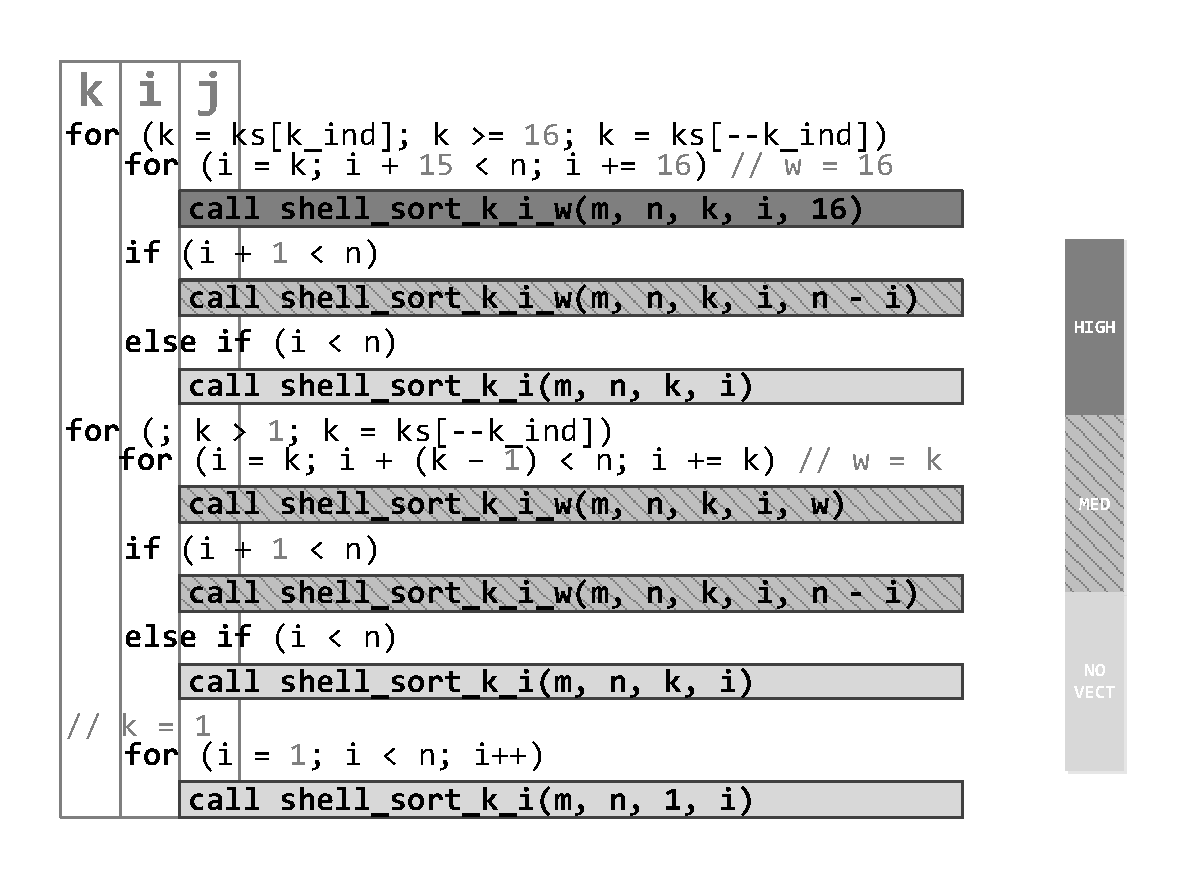
\includegraphics[width=0.65\textwidth]{pics/pic_decomposition.pdf}
\captionstyle{normal}\caption{Comparison of the theoretical acceleration of a vectorized version of Shell sorting for different sequences of steps}\label{pic:decompos}
\end{figure}

The $ shell\_sort\_k\_i\_w $ function, which appeared after decomposing the Shell sorting algorithm, contains the implementation of sorting $ w $ adjacent array slices, taken with step k. 
At the same time, the number of iterations of the inner loop of this function is unknown.
Moreover, the number of iterations of the inner loop when sorting one slice is in no way connected with the number of iterations of the inner loop when sorting the next slice.
This is a significant problem when attempting to merge the code for sorting adjacent slices using vector instructions.
For such a union, it is necessary to rewrite the slice sorting code in predicate form, then replace all instructions with vector analogs, and predicates with vector masks.
Moreover, if, prior to vectorization, the internal loop terminated when the predicate is false, then, after vectorization, the internal loop will terminate only if all elements of the corresponding vector mask are reset.
Thus, the number of iterations of the vectorized inner loop is equal to the maximum number of iterations of all $ w $ combined cycles.
If the values of the number of iterations of adjacent merged cycles differ greatly (and for Shell sorting this statement is true), then we get a loss of vectorization efficiency due to the low density of vector instruction masks (that is, a small percentage of vector elements is actually processed when performing vector operation).

Vectorized version of Shell sorting kernel presented in Listing \ref{lst:vectcode}. Also worth paying attention to the scatter operation, which appeared in the vector code, writing multiple data into memory with arbitrary offsets relative to the base address.
This command appeared as a vector analogue of a write operation to memory from the original code due to the same reason - the irregularity of the number of iterations of the internal loop.
It is worth noting that the scatter commands are extremely slow, which also causes a decrease in the efficiency of vectorization.

In addition to the designated scatter command, there are other memory reference commands in the vectorized code (Listing \ref{lst:vectcode}, lines 10, 16, 19).
These are the usual load and store commands that, generally speaking, must be addressed by aligned addresses in memory.
In the general case, the addresses given to them are certainly not aligned, however, the use of non-aligned calls instead of them significantly slows down the code, so it was decided to leave these instructions.

\begin{lstlisting}[caption={Vectorized version of Shell sorting kernel},label={lst:vectcode}]
void shell_sort_k_i_w(float *m, int n, int k, int i, int w)
{
    int j = i;
    __mmask16 ini_mask = ((unsigned int)0xFFFF) >> (16 - w);
    __mmask16 mask = ini_mask;
    __m512i ind_j = _mm512_add_epi32(_mm512_set1+epi32(i),
                                     ind_straight);
    __m512 t, q;
    
    t = _mm512_mask_load_ps(t, mask, &m[j]);

    do
    {
        mask = mask & _mm512_mask_cmp_epi32_mask(mask, ind_j, ind_k,
                                                 __MM_CMPINT_GE);
        q = _mm512_mask_load_ps(q, mask, &m[j - k]);
        mask = mask & _mm512_mask_cmp_ps_mask(mask, t, q,
                                              __MM_CMPINT_LT);
        _mm512_mask_store_ps(&m[j], mask, q);
        ind_j = _mm512_mask_sub_epi32(ind_j, mask, ind_j, ind_k);
        j -= k;
    }
    while (mask != 0x0);
    
    _mm512_mask_i32scatter_ps(m, ini_mask, ind_j, t, _MM_SCALE_4);
}
\end{lstlisting}

\subsection*{Theoretical acceleration calculation}

By theoretical acceleration, we will simply mean the ratio of the number of iterations of the internal cycle of the non-vectorized version to the one in the optimized vectorized version of the code.
Define this acceleration more formally.

First consider the non-vectorized code.
Denote by $ I (k, i) $ the number of iterations of the inner loop with fixed $ k $ and $ i $.
Then it is not difficult to calculate the total number of iterations of the inner loop when performing sorting (we denote this value as T).

\begin{equation}
T = \sum_{k \in ks}{\sum_{i = k}^{n - 1}{I(k, i)}}
\end{equation}

Now consider the vectorized version of the code. We also denote by $ I_v (k, i) $ the number of iterations of the inner loop with fixed $ k $ and $ i $.
We know that the vectorization width cannot exceed $ k $ (due to dependencies on accessing the array), and 16 (vector size), that is, $ w (k) = min (k, 16) $.
Moreover, the entire range of $ i $ values from $ k $ to $ n - 1 $, whose length is $ n - k $ is divided into $ \lfloor \frac {n - k} {w (k)} \rfloor $ groups in $ w $ elements in each, and the number of iterations in the vectorized cycle for each group is equal to the maximum value of the iterations of the non-vectorized cycles combined into this vectorized cycle.
Taking into account the vectorization of the tail part of the loop, we obtain the following formula for the total number of iterations of a vectorized inner loop.

\begin{equation}
T_v = \sum_{k \in ks}
{
\left(
\left(
\sum_{g = 0}^{G(k) - 1}{\max_{i = k + w(k)g}^{k + w(k)(g + 1) - 1}{I(k, i)}}
\right)
+ \max_{i = k + w(k)G(k)}^{n - 1}{I(k, i)}
\right)
}
\end{equation}

where $ w (k) = \min (k, 16) $, $ G (k) = \lfloor \frac {n - k} {w (k)} \rfloor $. The values of $ T = T (n) $ and $ T_v = T_v (n) $ were calculated when sorting pseudo-random arrays with the number of elements from 10 thousand to 2 million for each of the sequences of steps of Shell, Hibbard, Pratt and Sedgewick. 
Based on this, the theoretical acceleration $ s (n) = T (n) / T_v (n) $ was calculated. 
In addition, similar characteristics were calculated without taking into account the step $ k = 1 $ (these values are denoted $ T '(n) $, $ T'_v (n) $ and $ s' (n) $, respectively). 
The results were compared with the results of experimental launches on Intel Xeon Phi 7290 KNL microprocessor.


On the Fig.\ref{fig:theor_accel} and Fig.\ref{experim_accel} the results of theoretical estimates and experimental launches are presented. 
The figures show the dependence of vectorization efficiency on number of elements for Sedgwick, Pratt and Hibbard step sequences. 
It can be seen from the figures that even theoretical acceleration is far from ideal upper limit (equal to 16) of the acceleration achieved when vectorizing nested loops with a regular number of iterations. The experimental results, as was expected, are much lower and, finally, theoretical acceleration of Shell sorting barely exceeds the  2 mark. 

\begin{figure}[h]
\setcaptionmargin{5mm}
%\onelinecaptionsfalse % if the caption is multiline
\onelinecaptionstrue  % if the caption is one-line
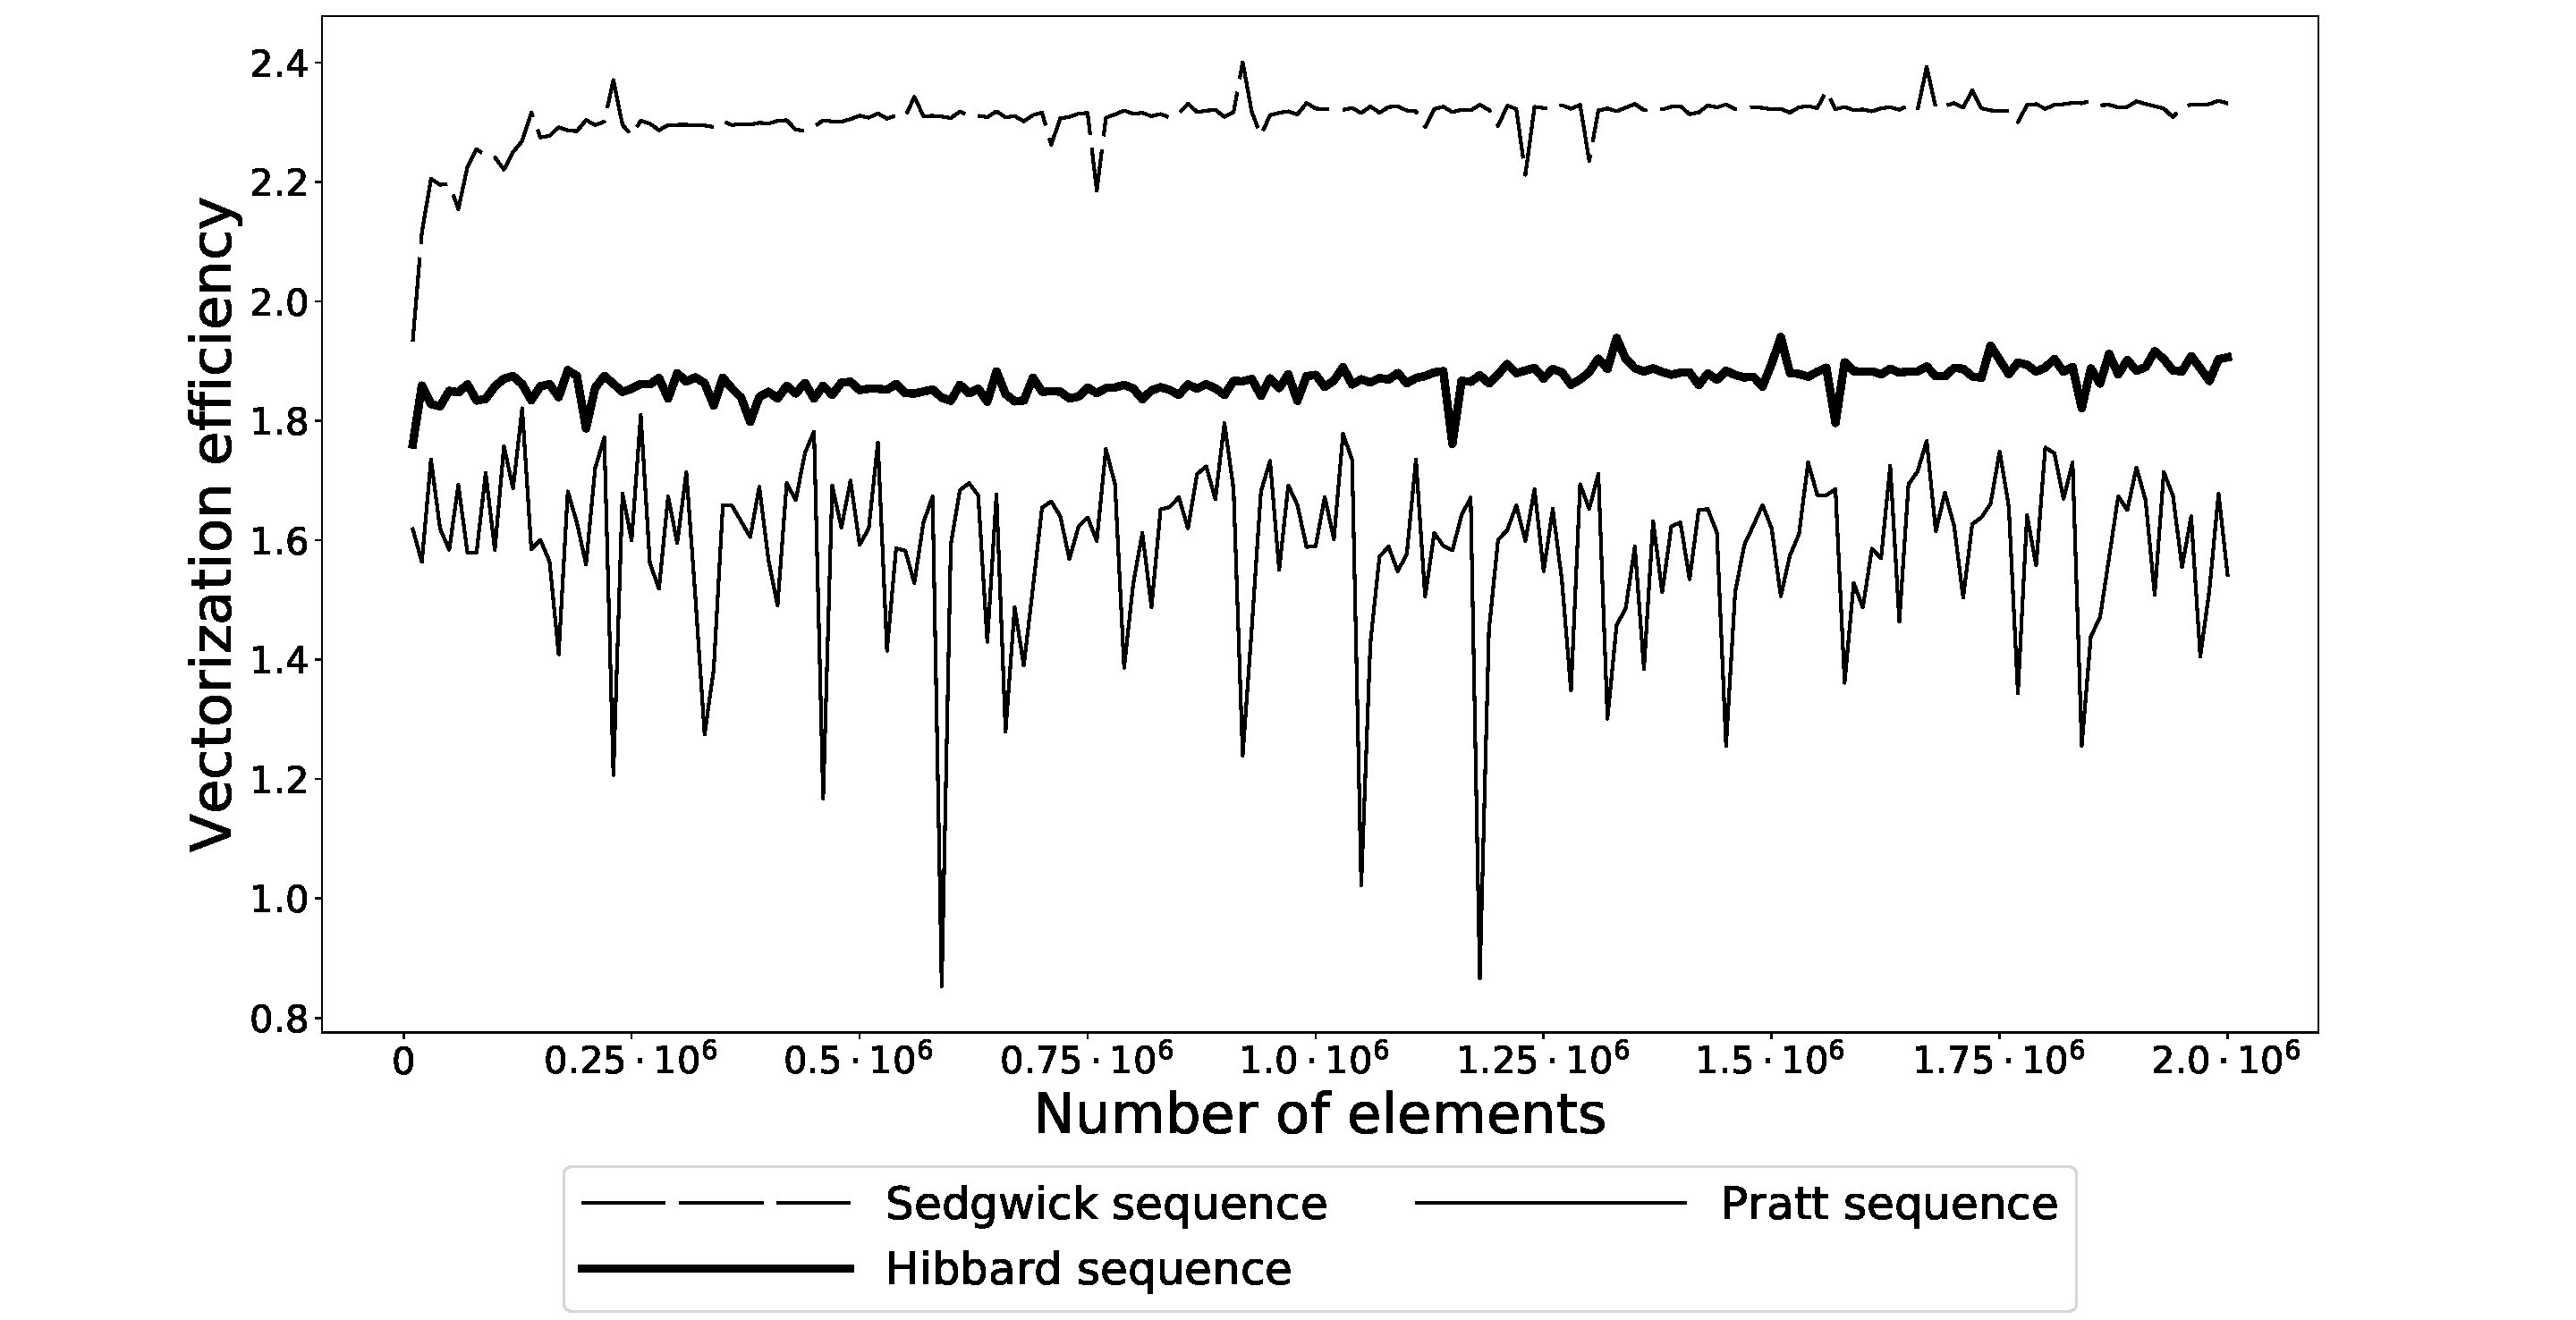
\includegraphics[width=0.85\textwidth]{pics/experimental_eff.pdf}
\captionstyle{normal}\caption{Comparison of the theoretical acceleration of a vectorized version of Shell sorting for different sequences of steps}\label{fig:theor_accel}
\end{figure}

\begin{figure}[h]
\setcaptionmargin{5mm}
%\onelinecaptionsfalse % if the caption is multiline
\onelinecaptionstrue  % if the caption is one-line
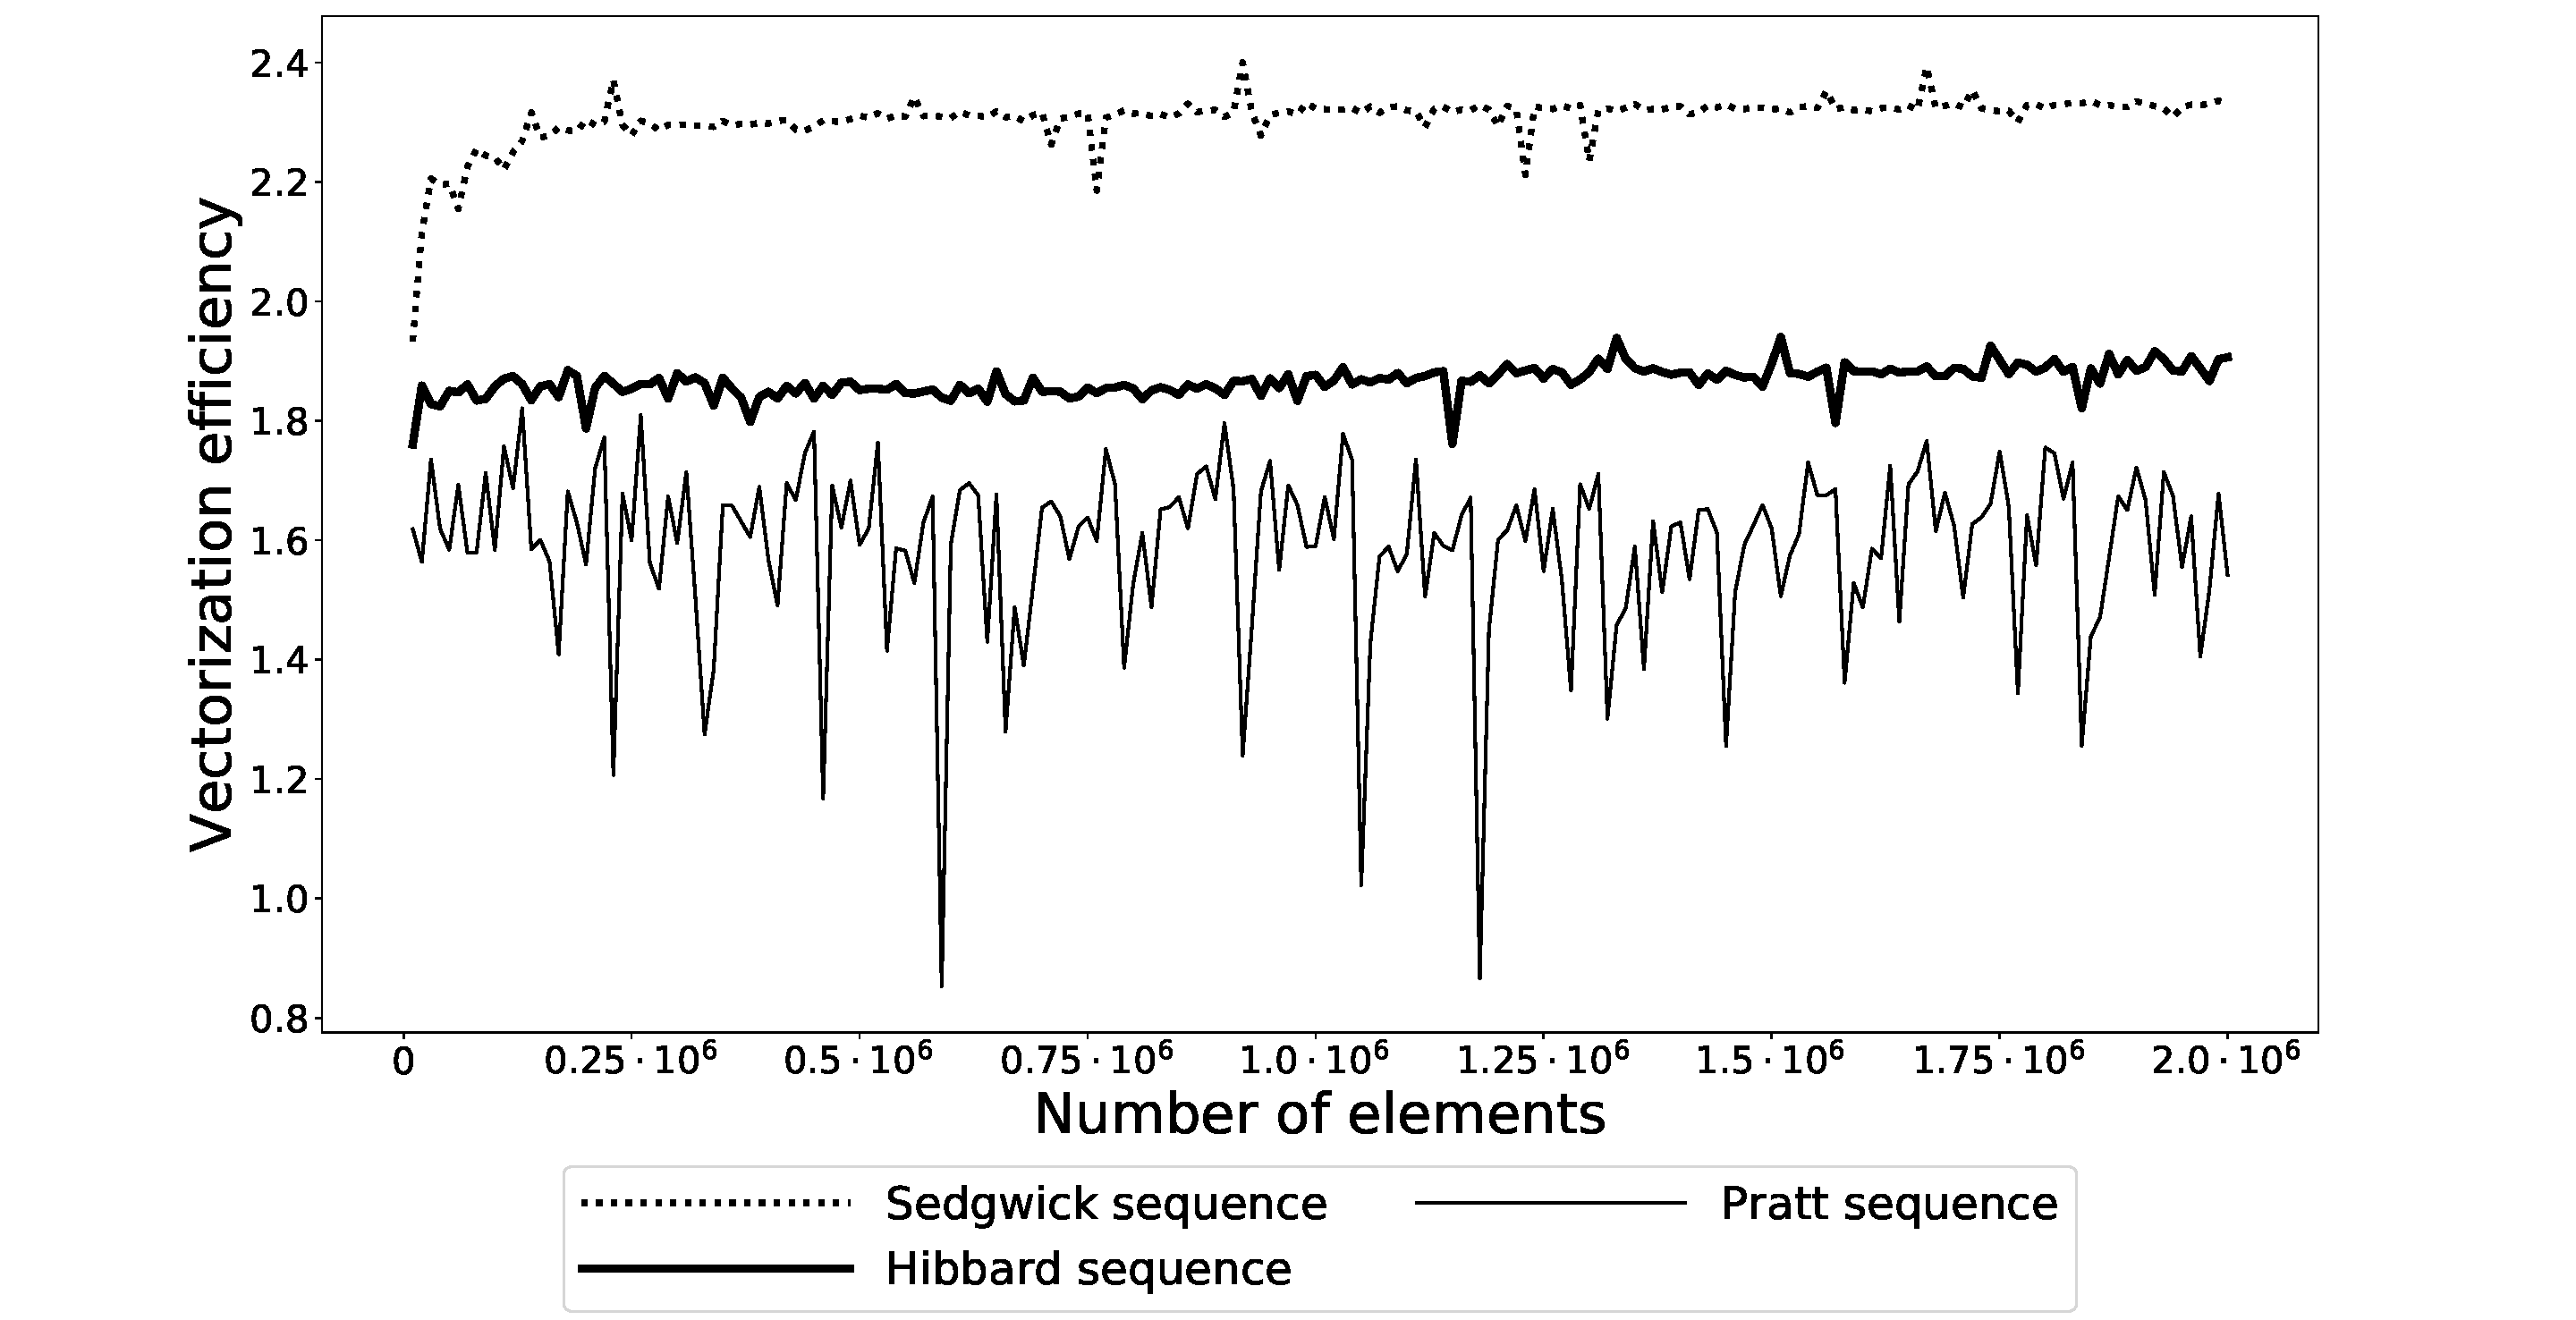
\includegraphics[width=0.85\textwidth]{pics/theoretical_eff.pdf}
\captionstyle{normal}\caption{Comparison of experimental acceleration of a vectorized version of Shell sorting for different sequences of steps}\label{experim_accel}
\end{figure}
        
\section{Physical calculations vectorization}

The implementation of the Riemannian solver considered in this article is publicly available on the Internet as part of the NUMERICA \ cite {Numerica} library. In this case, we will be interested in the one-dimensional case for a single-component medium, implemented as a pure function (function without side effects), which, by the density, velocity and gas pressure values to the left and right of the discontinuity, finds the values of the same quantities on the discontinuity itself at zero time time after removal of the septum.

\begin{equation}\label{eq:riemann}
U_l = \left( \begin{array}{ccc} d_l \\ u_l \\ p_l \end{array} \right),
U_r = \left( \begin{array}{ccc} d_r \\ u_r \\ p_r \end{array} \right),
U = \left( \begin{array}{ccc} d \\ u \\ p \end{array} \right) = riem(U_l, U_r)
\end{equation}

The NUMERICA library is implemented in the FORTRAN programming language, therefore the vectorization of this code using intrinsic functions is not directly possible, so the version of the code ported to the C programming language was used.

\begin{figure}[h]
\setcaptionmargin{5mm}
%\onelinecaptionsfalse % if the caption is multiline
\onelinecaptionstrue  % if the caption is one-line
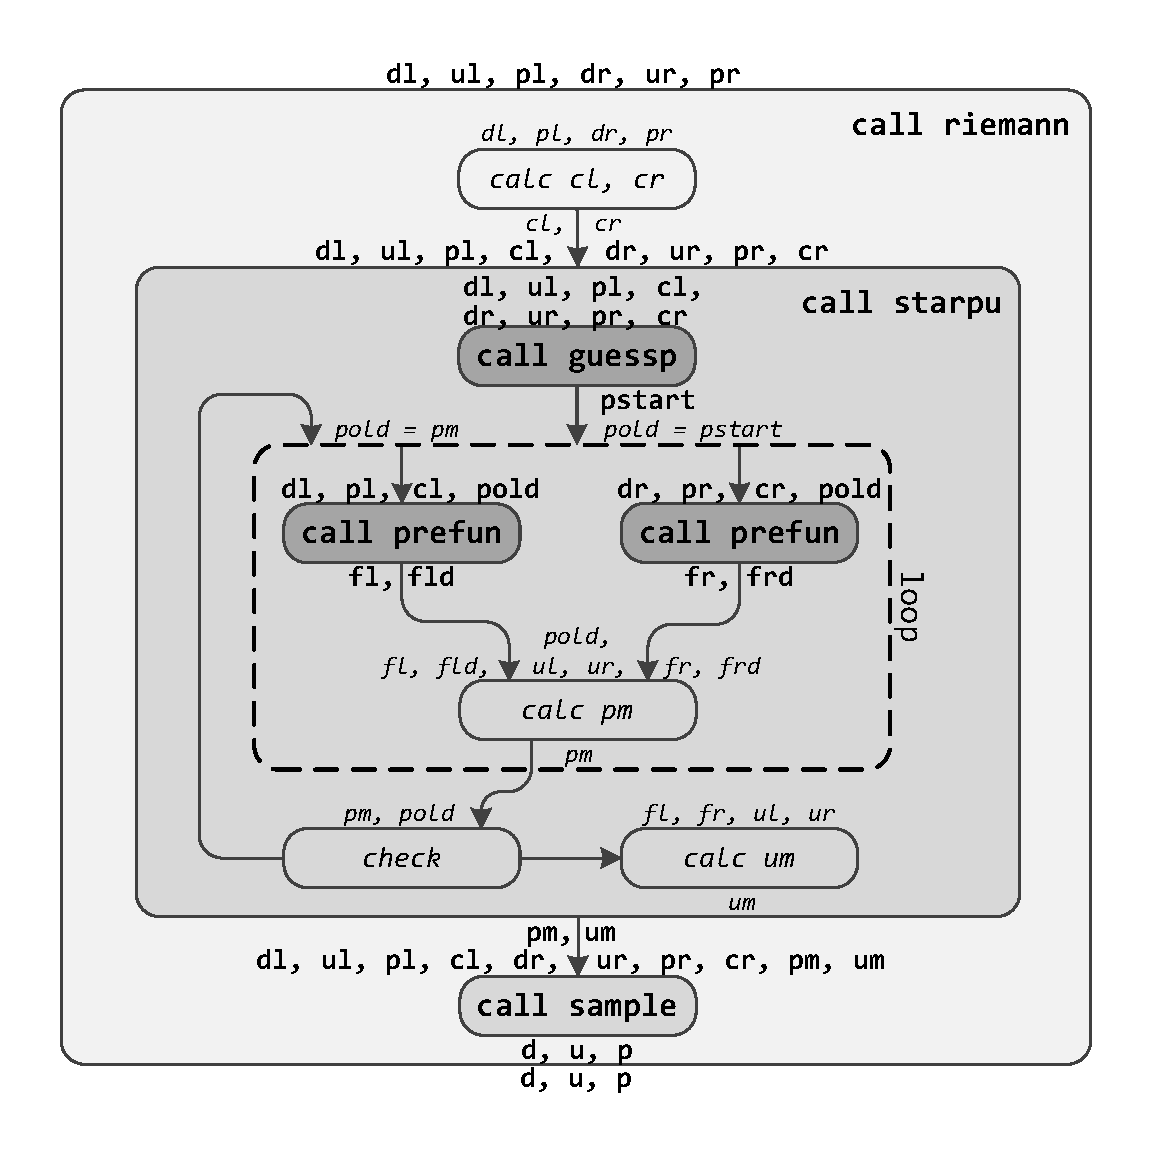
\includegraphics[width=0.6\textwidth]{pics/riemann.pdf}
\captionstyle{normal}\caption{Please write your figure caption here.}\label{fig:1}
\end{figure}

In Fig. ~ \ Ref {pic: functions} the scheme of work of the Riemannian solver with the indicated data streams and calls of all functions included in the implementation is shown. The riemann function calculates the speed of sound on the right and left, performs a vacuum test and successively calls the starpu and sample functions. The starpu function calculates the velocity and pressure values ​​in the middle region between the left and right waves (star region), and the function contains a cycle with an unknown number of iterations to solve a nonlinear equation using the Newton iterative method, inside which there are calls to other functions (prefun). The guessp and prefun functions contain only arithmetic calculations and simple conditions and are the simplest from the point of view of vectorization. Finally, the last sample function determines the final configuration of the discontinuity by calculating a set of conditions. This function contains a very extensive control, the nesting of conditions in it reaches four, which makes it difficult to use vectorization.

In the counting process, numerous riemann function calls are made with different input data sets using numerical methods based on the Riemannian solver (each call iteration makes one call for each face of each cell of the computational grid). Since the riemann function is pure, calls for different input data sets (dl, ul, pl, dr, ur, pr) are independent and there is a desire to combine calls with the goal of effectively using vector (element) instructions. As such a combined call, we will consider a function into which, instead of atomic data of the float type, the corresponding vectors containing 16 elements each are fed.

\begin{equation}\label{eq:riemann_16}
\overline{U_l} = \left( \begin{array}{ccc} U_l^1 \\ ... \\ U_l^{16} \end{array} \right),
\overline{U_r} = \left( \begin{array}{ccc} U_r^1 \\ ... \\ U_r^{16} \end{array} \right),
\overline{U} = \left( \begin{array}{ccc} U^1 \\ ... \\ U^{16} \end{array} \right) = riem^{16}(\overline{U_l}, \overline{U_r})
\end{equation}

At the same time, it is possible to perform the same actions with vector data as with basic types - perform calculations, transfer to functions, and return as a result. In the process of optimization, for clarity, it will avoid substitution of the function body into the call point. Thus, as a result of vectorization, our goal is to obtain the vector analogs of all the functions described above used in the Riemannian solver.

The sample function contains a highly branched control with a nesting level of 4 (see Fig. ~). The condition tree constructed for this function contains 10 leaf nodes, in each of which the value of the gas-dynamic quantities d, u, p is determined. Direct computation of the vector predicates of all leaf nodes and the execution of their code under these predicates leads to a slowdown of the resulting code, therefore, the following actions were performed when vectoring this function.

First, it was noted that the 4 linear sections contain the definition of the gas-dynamic parameters d, u, and p, which could be changed to initialization by moving the assignment operations up through the function code. Thus, 4 linear sections were deleted. At the same time, this initialization of the d, u, p parameters does not contain arithmetic operations (the parameters are initialized by the arguments of the function dl, ul, pl or dr, ur, pr), which means it can be performed using the vector merge operations blend.

It was further noted that the sample function processes the right and left profiles of the breakup decay in the same way with minor changes. Using a simple change of variables, which consists in changing the sign of the velocity value, we merged the code for two subtrees based on the condition pm $ \ le $ pl, which reduced the amount of the calculation code by half and expectedly reduced the execution time by 45%.

After the reduction of the code, the number of leaf nodes in the conditions tree was reduced to three. However, even in this case, direct merging of the code using vector predicates turned out to be ineffective. This was due to the unlikely part of the code, heavy operations, among which there are calls to the function of raising to a power (Fig. ~ \ Ref {pic: sample}, lines 033-036). The vector predicate of this code segment in more than 95 percent of cases has a value of 0x0, therefore, before executing this code section, it is advisable to check this predicate for emptiness (which corresponds to removing the unlikely branch of execution from the function body). The removal of an unlikely branch of execution from the main program context can significantly speed up the executable code, since the presence of a large number of such rare computations can serve as a reason for refusing vectorization \ cite {RybLowProb}.

For the rest of the code, you can merge with the comments described in the previous section. As a result, the vectorized sample function was accelerated more than 10 times. The final vector code is presented in Fig. ~ \ Ref {pic: }. In this code, lines 11–14 correspond to initialization, lines 16, 17, and 50 are responsible for replacing the variables for merging symmetric sections of the code, and the unlikely branch is selected in the block located in lines 41–47.

The approaches to the vectorization of the Riemann solver functions described in the article were implemented in the C programming language using functions intrinsikov and tested on microprocessors Intel Xeon Phi 7290, which are part of the computational segment knl supercomputer MVS-10P, located in the MSC RAS.

Performance testing was performed on the input data arrays collected in solving standard test problems: the Soda problem, the Lax problem, the weak shock wave problem, the Einfeldt problem, the Woodward-Colella problem, the Schu-Osher problem and others \ cite {BulVolTest}. As a result of the executed transformations of the source code, the Riemann solver accelerated by 7 times compared to the non-optimized versions.

\section{Conclusion}

conclusion

\begin{acknowledgments}
We thank A.~A.~Surname1 and B.~B.~Surname2 for their participation in discussions of the results. We are grateful to C.~C.~Surname3 and the reviewers for careful reading of the manuscript and helpful remarks. Links to grants are also listed here.
\end{acknowledgments}

\begin{thebibliography}{99}

% References for INTRODUCTION section.

% References for FLAT CYCLES section.

% References for MATRICES section.

\bibitem{Lyub_RANS_ILES}
\refitem{article}
D.~A.~Lyubimov, \textquotedblleft Development and Application of a High-Resolution Technique for Jet Flow Computation Using Large Eddy Simulation \textquotedblright, High Temperature, Vol.~50, No.~\textbf{3}, pp.~420-436 (2012).

\bibitem{Ben_Lyub_Chest_RANS_ILES}
\refitem{article}
L.~A.~Benderskii, D.~A.~Lyubimov, A.~O.~Chestnykh, B.~M.~Shabanov and A.~A.~Rybakov, \textquotedblleft The Use of the RANS/ILES Method to Study the Influence of Coflow Wind on the Flow in a Hot, Nonisobaric, Supersonic Airdrome Jet during Its Interaction with the Jet Blast Deflector \textquotedblright, High Temperature, Vol.~56, No.~\textbf{2}, pp.~247-254 (2018).

% References for IRREGULAR ITERATIONS LOOPS section.

% References for PHYSICAL CALCULATIONS section.

\bibitem{ex}
\refitem{article}
Rosales C. et al. (2016) A Comparative Study of Application Performance and Scalability on the Intel Knights Landing Processor. In: Taufer M., Mohr B., Kunkel J. (eds) High Performance Computing. ISC High Performance 2016. Lecture Notes in Computer Science, vol 9945. Springer, Cham

\bibitem{ex}
\refitem{article}
Newburn C.J., Sukha J., Sharapov I., Nguyen A.D., Miao CC. (2016) Application Suitability Assessment for Many-Core Targets. In: Taufer M., Mohr B., Kunkel J. (eds) High Performance Computing. ISC High Performance 2016. Lecture Notes in Computer Science, vol 9945. Springer, Cham

\bibitem{ex}
\refitem{article}
Doerfler D. et al. (2016) Applying the Roofline Performance Model to the Intel Xeon Phi Knights Landing Processor. In: Taufer M., Mohr B., Kunkel J. (eds) High Performance Computing. ISC High Performance 2016. Lecture Notes in Computer Science, vol 9945. Springer, Cham

\bibitem{ex}
\refitem{article}
Krzikalla O., Wende F., Hohnerbach M. (2016) Dynamic SIMD Vector Lane Scheduling. In: Taufer M., Mohr B., Kunkel J. (eds) High Performance Computing. ISC High Performance 2016. Lecture Notes in Computer Science, vol 9945. Springer, Cham

\bibitem{ex}
\refitem{article}
Malas T., Kurth T., Deslippe J. (2016) Optimization of the Sparse Matrix-Vector Products of an IDR Krylov Iterative Solver in EMGeo for the Intel KNL Manycore Processor. In: Taufer M., Mohr B., Kunkel J. (eds) High Performance Computing. ISC High Performance 2016. Lecture Notes in Computer Science, vol 9945. Springer, Cham

\bibitem{ex}
\refitem{article}
Walden A., Khan S., Joó B., Ranjan D., Zubair M. (2016) Optimizing a Multiple Right-Hand Side Dslash Kernel for Intel Knights Corner. In: Taufer M., Mohr B., Kunkel J. (eds) High Performance Computing. ISC High Performance 2016. Lecture Notes in Computer Science, vol 9945. Springer, Cham

\bibitem{ex}
\refitem{article}
Deslippe J. et al. (2016) Optimizing Excited-State Electronic-Structure Codes for Intel Knights Landing: A Case Study on the BerkeleyGW Software. In: Taufer M., Mohr B., Kunkel J. (eds) High Performance Computing. ISC High Performance 2016. Lecture Notes in Computer Science, vol 9945. Springer, Cham

\bibitem{ex}
\refitem{article}
Joó B., Kalamkar D.D., Kurth T., Vaidyanathan K., Walden A. (2016) Optimizing Wilson-Dirac Operator and Linear Solvers for Intel® KNL. In: Taufer M., Mohr B., Kunkel J. (eds) High Performance Computing. ISC High Performance 2016. Lecture Notes in Computer Science, vol 9945. Springer, Cham

\bibitem{ex}
\refitem{article}
Al Hasib, A., Cebrian, J.M. \& Natvig, L. J Supercomput (2018) 74: 2705. https://doi.org/10.1007/s11227-018-2310-0.

\bibitem{ex}
\refitem{article}
Bramas, B. Fast sorting algorithms using AVX-512 on Intel Knights Landing. arXiv: 1704.08579 [cs. MS]. URL: https://arxiv.org/abs/1704.08579 (visited on 10.11.2018).

\bibitem{ex}
\refitem{article}
Watanabe H., Nakagawa K. M. SIMD Vectorization for the Lennard-Jones Potential with AVX2 and AVX-512 instructions. arXiv:1806.05713 [cs. MS]. URL: https://arxiv.org/abs/1806.05713 (visited on 12.10.2018).

\bibitem{ex}
\refitem{article}
Bramas, B. A Novel Hybrid Quicksort Algorithm Vectorized using AVX-512 on Intel Skylake In: International Journal of Advanced Computer Science and Applications(IJACSA), Vol. 8 No. 10 2017.

\bibitem{ex}
\refitem{article}
Bramas, B. Increasing the Degree of Parallelism Using Speculative Execution in Task-based Runtime Systems. arXiv:1803.04211 [cs.DC]. URL: https://arxiv.org/abs/1803.04211 (visited on 12.10.2018).

\bibitem{ex}
\refitem{article}
Bramas B, Kus P. (2018) Computing the sparse matrix vector product using block-based kernels without zero padding on processors with AVX-512 instructions. PeerJ Computer Science 4:e151 https://doi.org/10.7717/peerj-cs.151

\bibitem{ex}
\refitem{article}
Messner, M., Bramas, B., Coulaud, O., Darve E. Optimized M2L Kernels for the Chebyshev Interpolation based Fast Multipole Method. arXiv:1210.7292 [cs.NA]. URL: https://arxiv.org/abs/1210.7292 (visited on 12.10.2018).

\bibitem{ex}
\refitem{article}
Hong Zhang, Richard T. Mills, Karl Rupp, and Barry F. Smith. 2018. Vectorized Parallel Sparse Matrix-Vector Multiplication in PETSc Using AVX-512. In Proceedings of the 47th International Conference on Parallel Processing (ICPP 2018). ACM, New York, NY, USA, Article 55, 10 pages. DOI: https://doi.org/10.1145/3225058.3225100.

\bibitem{ex}
\refitem{article}
Kulikov, I.M., Chernykh, I.G., Glinskiy, B.M. et al. Lobachevskii J Math (2018) 39: 543. https://doi.org/10.1134/S1995080218040091

\bibitem{ex}
\refitem{article}
Lim, R., Lee, Y., Kim, R. et al. Cluster Comput (2018). https://doi.org/10.1007/s10586-018-2810-y

\bibitem{ex}
\refitem{article}
Shay Gueron, Vlad Krasnov; Fast Quicksort Implementation Using AVX Instructions, The Computer Journal, Volume 59, Issue 1, 1 January 2016, Pages 83–90, https://doi.org/10.1093/comjnl/bxv063

\bibitem{ex}
\refitem{article}
Ungethum, A., Pietrzyk, J., Damme, P., Habich, D., Lehner, W. (2018). Conflict detection-based run-length encoding - AVX-512 CD instruction set in action. Paper presented at the Proceedings - IEEE 34th International Conference on Data Engineering Workshops, ICDEW 2018, 96--101.

\bibitem{ex}
\refitem{article}
Aleen, F., Zakharin, V. P., Krishnaiyer, R., Gupta, G., Kreitzer, D., and Lin, C. -., Jr. (2018). Automated compiler optimization of multiple vector Loads/Stores. International Journal of Parallel Programming, 46(2), 471-503. doi:10.1007/s10766-016-0485-7

\bibitem{ex}
\refitem{article}
Jubertie, S., Dupros, F., and De Martin, F. (2018). Vectorization of a spectral finite-element numerical kernel. Paper presented at the WPMVP 2018 - Proceedings of the 2018 4th Workshop on Programming Models for SIMD/Vector Processing, Co-Located with PPoPP 2018, doi:10.1145/3178433.3178441

\bibitem{ex}
\refitem{article}
Jeffers J., Reinders J., Sodani A. Intel Xeon Phi processor high performance programming. Knights Land-ing Edition. Morgan Kaufmann Publ., 2016, 632 p.

\bibitem{ex}
\refitem{article}
Intel C++ Compiler 16.0 User and Reference Guide. Intel Corporation. 2015. URL: https://software.intel.com/en-us/articles/intel-c-compiler-160-for-windows-release-notes-for-intel-parallel-studio-xe-2016 (visited on 11.10.2018).

\bibitem{ex}
\refitem{article}
Intel Intrinsics Guide. URL: https://software.intel.com/sites/landingpage/IntrinsicsGuide (visited on 11.10.2018).

\bibitem{ex}
\refitem{article}
Krzikalla O., Wende F., Hohnerbach M. Dynamic SIMD Vector Lane Scheduling. In: ISC High Perfor-mance Workshops 2016, M. Taufer et al. (eds.), LNCS, 2016, vol. 9945, pp. 354 –- 365.

\bibitem{ex}
\refitem{article}
Cook B., Maris P., Shao M. High Performance Optimizations for Nuclear Physics Code MFDn on KNL. In: ISC High Performance Workshops 2016, M. Taufer et al. (eds.), LNCS, 2016, vol. 9945, pp. 366 -- 377.

\bibitem{ex}
\refitem{article}
Deslippe J., da Jornada F.H., Vigil-Fowler D. et al. Optimizing Excited-State Electronic-Structure Codes for Intel Knights Landing: A Case Study on the BerkeleyGW Software. In: ISC High Performance Workshops 2016, M. Taufer et al. (eds.), LNCS, 2016, vol. 9945, pp. 402 -- 414.

\bibitem{ex}
\refitem{article}
Maleki S., Gao Ya., Garzaram M.J., Wong T., Padua D.A. An evaluation of vectorizing compilers // Proc. Int. Conf. on Parallel Architectures and Compilation Techniques (PACT'11), 2011, pp. 372 -- 382.

\bibitem{ex}
\refitem{article}
LINKS TO https://oeis.org/A102549 FOR INTEGER SEQUENCES




\end{thebibliography}

\end{document}
